\documentclass[12pt, a4paper, twoside,titlepage]{article}

\usepackage{times}
\usepackage[cp1250]{inputenc}
\usepackage[T1]{fontenc}
\usepackage[polish]{babel}
\usepackage{setspace}
\usepackage{graphicx}
\usepackage{float}
\usepackage{subcaption}
%\usepackage{subfig}
\usepackage{enumerate}
\usepackage{wrapfig}
\usepackage{bm}
\usepackage{cite}
\usepackage{amsmath}
\usepackage{amsfonts}
\usepackage{cleveref}
\usepackage{indentfirst}
\usepackage[export]{adjustbox}
\usepackage{array}
\usepackage{booktabs}
\usepackage{fancyhdr}
\usepackage{multirow}

\pagestyle{fancy}
\fancyhf{}
\renewcommand{\headrulewidth}{0pt}
%\fancyfoot[CE,CO]{\leftmark}
\fancyfoot[LE,RO]{\thepage}

\numberwithin{equation}{section}


\hyphenpenalty=10000		% nie dziel wyraz�w zbyt cz�sto
\clubpenalty=10000			% kara za sierotki
\widowpenalty=10000			% nie pozostawiaj wd�w
\brokenpenalty=10000		% nie dziel wyraz�w mi�dzy stronami
\exhyphenpenalty=999999		% nie dziel s��w z my�lnikiem
\righthyphenmin=3			% dziel minimum 3 litery

\tolerance=4500
\pretolerance=250
\hfuzz=1.5pt
\hbadness=1450

\sloppy						% umacnia pozycj� prawego marginesu

\setlength{\textwidth}{\paperwidth}
\addtolength{\textwidth}{-5cm}
\setlength{\textheight}{\paperheight}
\addtolength{\textheight}{-5cm}
\setlength{\oddsidemargin}{0cm}
\setlength{\evensidemargin}{0cm}
\topmargin -1.25cm
\footskip 1.4cm

\graphicspath{ {./graph/}} 

\author{Micha� Jarzyna}
\title{Identyfikacja parametr�w ci�g�ego obiektu liniowego.}
\date{\today}

\newcommand{\pparagraph}[1]{\paragraph{#1}\mbox{}\\}
\newcommand{\subpparagraph}[1]{\subparagraph{#1}\mbox{}\\}


\begin{document}

\makeatletter
\begin{titlepage}
\center \Huge \@title
\center \normalsize \@author
\center \scriptsize \@date
\end{titlepage}
\makeatother
\newpage
%\thispagestyle{empty}
%\mbox{}
%\newpage

\newpage
\tableofcontents

\newpage
\section{Zadanie identyfikacyjne}

Proces do identyfikacji zadany jest nast�puj�cym r�wnaniem:
\begin{equation}\label{eq:obj}
\dot{y}(t) = -a\cdot y(t) +  u(t).
\end{equation}
Nale�y zaprojektowa� i zasymulowa� algorytm adaptacyjny postaci:
\begin{equation}\label{eq:alg}
\dot{k}(t) = f(y(t))
\end{equation}
s�u��cy do identyfikacji nieznanego parametru $a$ zak�adaj�c, �e sterowanie jest funkcj� odpowiedzi procesu:
\begin{equation}\label{eq:ster}
u(t) = g\left( y \left(t \right) \right),
\end{equation}
oraz gwarantuj�c jego stabilno��.










 
\newpage
\section{Wyznaczanie algorytmu}
Rozpoczynaj�c od tego rozdzia�u dla wszystkich uprzednio zdefiniowanych funkcji czasu zostaje pomini�ty jawny zapis zale�no�ci od czasu ($y(t) \rightarrow y$) w celu zwi�kszenia klarowno�ci zapisu.
\subsection{Za�o�enia uzupe�niaj�ce}
Stabilno�� obiektu wymaga spe�nienia warunk�w Hurwitza, w szczeg�lno�ci, dla zadanego obiektu warunek ten sprowadza si� do postaci:
\begin{equation}\label{eq:z1}
a>0.
\end{equation}

Za�o�ono wyst�powanie nieznanego parametru obiektu skaluj�cego wp�yw sterowania. Zmodyfikowane r�wnanie \ref{eq:obj} przyjmuje posta�:
\begin{equation}\label{eq:objb}
\dot{y} = -a\cdot y + b \cdot u
\end{equation}

Identyfikacji b�d� podlega� dwa parametry, wi�c algorytm identyfikacyjny (\ref{eq:alg}) przyjmie posta�:
\begin{equation}\label{eq:alg2}
\dot{k} =	\begin{bmatrix}
			\dot{\Theta}_1(t) \\ \\
			\dot{\Theta}_2(t)
		\end{bmatrix} = \begin{bmatrix}
			f_1(y(t)) \\ \\
			f_2(y(t))
		\end{bmatrix}
\end{equation}

\subsection{Model identyfikacyjny}
Identyfikacj� parametr�w zrealizowano poprzez zastosowanie referencyjnego obiektu liniowego:
\begin{equation}\label{eq:mod}
\dot{\hat{y}}(t) = -\hat{a} \hat{y}(t) + \hat {b} u_c(t), \hat{a} > 0.
\end{equation}

Wykorzystuj�c tak skonstruowany model i algorytm identyfikacji (\ref{eq:alg2}) sterowanie (\ref{eq:ster}) wyznaczono w nast�puj�cy spos�b:
\begin{equation}\label{eq:sterparam}
 u = \Theta_1u_c - \Theta_2  y.
\end{equation}

Zagwarantowanie r�wnowa�nego zachowania obiektu (\ref{eq:obj}) oraz modelu (\ref{eq:mod}) od momentu zr�wnania si� wyj�� obu obiekt�w $y = \hat{y}$  wymaga spe�nienia warunku:
\begin{align*}
\dot{y} &= \dot{\hat{y}} \\
-ay + bu &= -\hat{a}\hat{y}+\hat{b}u_c  & | u &= \Theta_1 u_c - \Theta_2  y\\
-ay + b(\Theta_1 u_c - \Theta_2  y) & =  -\hat{a}\hat{y}+\hat{b}u_c \\
\hat{a}\hat{y} - ay - b\Theta_2y & + b\Theta_1u_c - \hat{b}u_c = 0  &|y & =\hat{y}\\
y(\hat{a} - a -b\Theta_2) + u_c(b\Theta_1 - \hat{b}) & = 0 & |(y\not\equiv 0  &\land \hat{y}\not\equiv 0).
\end{align*}
Powy�szy warunek jest spe�niony, je�li parametry $\Theta$ przyjm� nast�puj�ce warto�ci:
\begin{equation}\label{eq:cond1}
\Theta_1 = \frac{\hat{b}}{b} \land \Theta_2 = \frac{\hat{a} - a}{b} .
\end{equation}
Ponadto r�nica pomi�dzy wyj�ciami obiektu i modelu jest nast�puj�ca:
\begin{equation}\label{eq:e}
e(t) = y - \hat{y}.
\end{equation}
Po��dany punkt stabilno�ci jest wi�c nast�puj�cej postaci:
\begin{equation}\label{eq:setpt}
x^* = 
\begin{bmatrix} 	e^* \\ \\
			\Theta_1^*\\ \\
			\Theta_2^*
\end{bmatrix} = \begin{bmatrix}
		0\\ \\
		\frac{\hat{b}}{b}\\ \\
		\frac{\hat{a}-a}{b}
\end{bmatrix}.
\end{equation}

\subsection{Algorytm identyfikacyjny}
Dysponuj�c po�adanym punktem stabilno�ci (\ref{eq:setpt}) mo�na zaproponowa� funkcj� Lapunowa w formie po�owy modyfikowanej normy $L_2$ wektora ��cz�cego bie��cy stan z po��danym:
\begin{equation}\label{eq:V}
V(e, \Theta_1, \Theta_2) = \frac{1}{2} \left[ e^2 + \frac{1}{\gamma b}\left( b\Theta_1 - \hat{b}\right) ^2 + \frac{1}{\gamma b} \left( b \Theta_2 - \left( \hat{a} - a\right) \right) ^2 \right].
\end{equation}

Warto�� tak skonstruowanej funkcji Lapunowa w punkcie $x_0$ wynosi:
\begin{equation}\label{eq:L1}
V(x^*) = \frac{1}{2} \left[ e^2 + \frac{1}{\gamma b}\left( b\frac{\hat{b}}{b} - \hat{b}\right) ^2 + \frac{1}{\gamma b} \left( b \frac{\hat{a}-a}{b} - \left( \hat{a} - a\right) \right) ^2 \right] = 0,
\end{equation}
wi�c spe�nia $1^\circ$ warunek twierdzenia Lapunowa o stabilno�ci.

Parametr $b$ jest nieznany, jednak znaj�c jego znak(dla obiektu liniowego parametr $b>0$ da odpowied� prost�, natomiast $b<0$ odpowied� odwrotn�; okre�lenie znaku wymaga wi�c jedynie jednego prostego eksperymentu) �atwo dobra� parametr $\gamma$ tak, �eby iloczyn $b\gamma > 0$. Tak dobrany parametr $\gamma$ sprawia, �e funkcja Lapunowa okre�lona r�wnaniem (\ref{eq:V}) jest sum� kwadrat�w zmiennych wa�on� dodatnimi parametrami, a wi�c dla dowolnych zmiennych niezeruj�cych ca�ego wyra�enia warto�� tej funkcji b�dzie dodatnia. To spostrze�enie gwarantuje spe�nienie $2^\circ$ warunku twierdzenia Lapunowa o stabilno�ci.

$3^\circ$ warunku twierdzenia Lapunowa o stabilno�ci wymaga wyznaczenia pochodnej funkcji Lapunowa po czasie:
\begin{align*}
\dot{V}(e, \Theta_1, \Theta_2) &= e\dot{e} + \frac{1}{\gamma}\left( b\Theta_1 - \hat{b}\right)\dot{\Theta}_1 + \frac{1}{\gamma}\left( b\Theta_2 - \left( \hat{a} - a \right) \right) \dot{\Theta}_2\\
/\dot{e} &= \dot{y} - \dot{\hat{y}}  & | \dot{y} & = -ay+bu  \land \dot{\hat{y}} =-\hat{a}\hat{y} + \hat{b}u_c /\\
/\dot{e} &= -ay+bu - (-\hat{a}\hat{y} + \hat{b}u_c) & |u &= \Theta_1 u_c - \Theta_2 y / \\
/\dot{e} &=-ay + b( \Theta_1 u_c - \Theta_2 y) + \hat{a}\hat{y} - \hat{b}u_c + 0& | 0& =\hat{a}y - \hat{a}y/\\
/\dot{e} &= -ay + b\Theta_1 u_c - b\Theta_2 y + \hat{a}\hat{y} - \hat{b}u_c +\hat{a}y - \hat{a}y/\\
/\dot{e} &= -\hat{a}(y - \hat{y}) + (b\Theta_1 - \hat{b})u_c + (\hat{a} - a - b\Theta_2)y& | e&=y - \hat{y}/ \\
/e\dot{e}&= -\hat{a}e^2 + (b\Theta_1 - \hat{b})u_ce + (\hat{a} - a - b\Theta_2)ye/ 
\end{align*}
\begin{align*}
\dot{V} & =-\hat{a}e^2 + (b\Theta_1 - \hat{b})u_ce + (\hat{a} - a - b\Theta_2)ye + \frac{1}{\gamma}\left( b\Theta_1 - \hat{b}\right)\dot{\Theta}_1 + \frac{1}{\gamma}\left( b\Theta_2 - \left( \hat{a} - a \right) \right) \dot{\Theta}_2 
\end{align*}
\begin{equation}\label{eq:dV}
\dot{V} = -\hat{a}e^2 +  (b\Theta_1 - \hat{b})\left(  \frac{\dot{\Theta}_1 }{\gamma} + u_ce\right) + \left( b\Theta_2 - \left( \hat{a} - a \right) \right) \left( \frac{\dot{\Theta}_2}{\gamma} - ye  \right)
\end{equation}
Spe�nienie $3^\circ$ warunku twierdzenia Lapunowa o stabilno�ci wymaga, aby warto�� wyra�enia (\ref{eq:dV}) by�a ujemna wsz�dzie poza punktem stabilno�ci. Wyraz $-\hat{a}e^2$ spe�nia ten warunek zawsze, ze wzgl�du na za�o�enia (\ref{eq:mod}). Mo�na wp�ywa� na warto�ci $\dot{\Theta}_1$ i $\dot{\Theta}_2$, a wi�c najprostsz� metod� zapewnienia wymaga�  $3^\circ$ warunku twierdzenia Lapunowa o stabilno�ci jest wyzerowanie pozosta�ych wyraz�w wyra�enia (\ref{eq:dV}) w nast�puj�cy spos�b:
\begin{equation}\label{eq:dTh}
\begin{bmatrix}
\dot{\Theta}_1\\ \\
\dot{\Theta}_2
\end{bmatrix} = 
\begin{bmatrix}
-u_ce\gamma\\ \\
ye\gamma
\end{bmatrix}.
\end{equation}

Dysponuj�c metod� wyznaczania parametru $\gamma$ powy�sze wyra�enie jest gotowym algorytmem identyfikuj�cym zadane parametry. Gdy warto�� $e$ ustabilizuje si� w 0, to poszukiwane parametry procesu mo�na odczyta� w nast�puj�cy spos�b:
\begin{equation}\label{eq:read}
\begin{bmatrix}
a_{est}\\ \\
b_{est}
\end{bmatrix}=
\begin{bmatrix}
\hat{a} - \hat{b}\frac{\Theta_2}{\Theta_1}\\ \\
\frac{\hat{b}}{\Theta_1} 
\end{bmatrix}
\end{equation}


 

\newpage
\section{Symulacja algorytmu identyfikacyjnego}
Symulacj� zaprojektowanego algorytmu przeprowadzono za pomoc� pakietu MATLAB.
\subsection{Symulowany uk�ad}
Uk�ad r�wna� r�niczkowych opisuj�cych uk�ad wraz z algorytmem identyfikacyjnym sk�ada si� z r�wna� (\ref{eq:obj}), (\ref{eq:mod}), (\ref{eq:e}) oraz (\ref{eq:dTh}) i wyra�a si� w nast�puj�cy spos�b:
\begin{equation}
\begin{bmatrix}
\dot{y} \\ \\ 
\dot{\hat{y}} \\ \\
\dot{e} \\ \\
\dot{\Theta}_1 \\ \\
\dot{\Theta}_2
\end{bmatrix} = 
\begin{bmatrix}
-ay + bu \\ \\
-\hat{a}\hat{y} + \hat{b}u_c \\ \\
\dot{y} - \dot{\hat{y}} \\ \\
-u_ce\gamma \\ \\
ye\gamma
\end{bmatrix} = \left| u =  \Theta_1 u_c - \Theta_2y \right| =
\begin{bmatrix}
-ay + b \Theta_1 u_c - b\Theta_2y \\ \\
-\hat{a}\hat{y} + \hat{b}u_c \\ \\
\dot{y} - \dot{\hat{y}} \\ \\
-u_ce\gamma \\ \\
ye\gamma
\end{bmatrix}.
\end{equation}
W uk�adzie tym wyst�puj� nast�puj�ce obiekty:
\begin{itemize}
\item zmienne stanu: $[y, \hat{y}, e, \Theta_1, \Theta_2]^{T}$ (nie wyst�puj� przekszta�cenia mi�dzy stanem, a wyj�ciem, wi�c mo�na je traktowa� jako to�same),
\item sygna� steruj�cy $[u_c]$,
\item parametry znane: $[\hat{a}, \hat{b}, \gamma]$,
\item parametry nieznane: $[a, b]$.
\end{itemize}
Sygna� $e$ jest wyznacznikiem realizacji zadania identyfikacji, jednak �atwo go wyrugowa� z r�wna�, a nast�pnie ponownie wyznaczy� na podstawie pozosta�ych przebieg�w. Dodatkowo zmniejszenie uk�adu r�wna� przyspieszy obliczenia (w tym przypadku nieznacznie, ale w og�lno�ci warto si� o to stara�). Zmodyfikowany uk�ad przyjmie posta�:
\begin{equation}\label{eq:sym}
\begin{bmatrix}
\dot{y} \\ \\ 
\dot{\hat{y}} \\ \\
\dot{\Theta}_1 \\ \\
\dot{\Theta}_2
\end{bmatrix} = 
\begin{bmatrix}
-ay + b \Theta_1 u_c - b\Theta_2y \\ \\
-\hat{a}\hat{y} + \hat{b}u_c \\ \\
-u_c({y} - {\hat{y}})\gamma \\ \\
y({y} - {\hat{y}})\gamma
\end{bmatrix}.
\end{equation}
Uzyskany uk�ad sk�ada si� z r�wna� r�niczkowych pierwszego rz�du i jako taki nie wymaga dalszych modyfikacji przed implementacj�. Aspekty, kt�re wymagaj� komentarza s� nast�puj�ce:
\begin{itemize}
\item stan pocz�tkowy $x_0 = [y_0, \hat{y}_0, \Theta_{10}, \Theta_{20}]^{T}$ b�dzie generowany w nast�puj�cy spos�b:
$y_0$  losowe - nie ma powodu zak�ada� czegokolwiek o nieznanym obiekcie, $\hat{y}_0 = 0$ w obiekcie nie wyst�puje wyraz ${\sim \frac{1}{\hat{y}}}$, wi�c to bezpieczny punkt sartowy, $ \Theta_{10} = 1$  optymistyczne za�o�enie, �e obiekt i model maj� takie same parametry $b$, $ \Theta_{20} = 0$ optymistyczne za�o�enie, �e obiekt i model maj� r�wne parametry $a$;
\item parametry nieznane $[a, b]$ b�d� losowane;
\item parametry znane $[\hat{a}, \hat{b}]$ b�d� wybierane jako $[1 1]$ - najprostszy nietrywialny obiekt, natomiast parametr $\gamma$ b�dzie okre�lony jako ${\gamma=sign(b)}$, w celu spe�nienia za�o�enia $b\gamma > 0$.
\end{itemize}

\subsection{Sygna� steruj�cy}
Analizuj�c uk�ad r�wna� (\ref{eq:sym}) wida�, �e pochodne sygna��w identyfikuj�cych $\dot{\Theta}_1, \dot{\Theta}_2$ s� zale�ne liniowo od r�nicy pomi�dzy wyj�ciami obiektu i modelu $e = y - \hat{y}$, w szczeg�lno�ci, gdy wyraz $e = 0$ nadmienione pochodne zeruj� si�, co oznacza, �e algorytm adaptacyjny zatrzyma si�. Wyzerowanie si� sygna�u $e$ mo�e nast�pi� w dw�ch przypadkach: identyfikacja obiektu zako�czy�a si� sukcesem, albo sygna�y $y$ i $\hat{y}$ ustali�y si� na r�wnym poziomie ze wzgl�du na sta�o�� sterowania $u_c$, jednak parametry $\Theta_1, \Theta_2$ zidentyfikowa�y inny obiekt liniowy, kt�ry dla sterowania $u = \Theta_1 u_c -  \Theta_2 y$ ustala si� akurat na tym samym poziomie (istnieje niesko�czenie wiele takich obiekt�w liniowych dla zadanego poziomu). Zabezpieczenie si� przed zagro�eniem zaj�cia drugiej sytuacji wymaga zmienno�ci sygna�u steruj�cego $u_c$ w czasie. Z tego wzgl�du zaproponowano sinusoidalny przebieg sygna�u steruj�cego $u_c = \sin(t)$.

\subsection{Przyk�adowa symulacja}
Przygotowany projekt symuluje algorytm identyfikacji nieznanych parametr�w obiektu liniowego. Poni�ej przedstawiono przyk�adowy wynik symulacji:
\begin{figure}[H]
\begin{center}
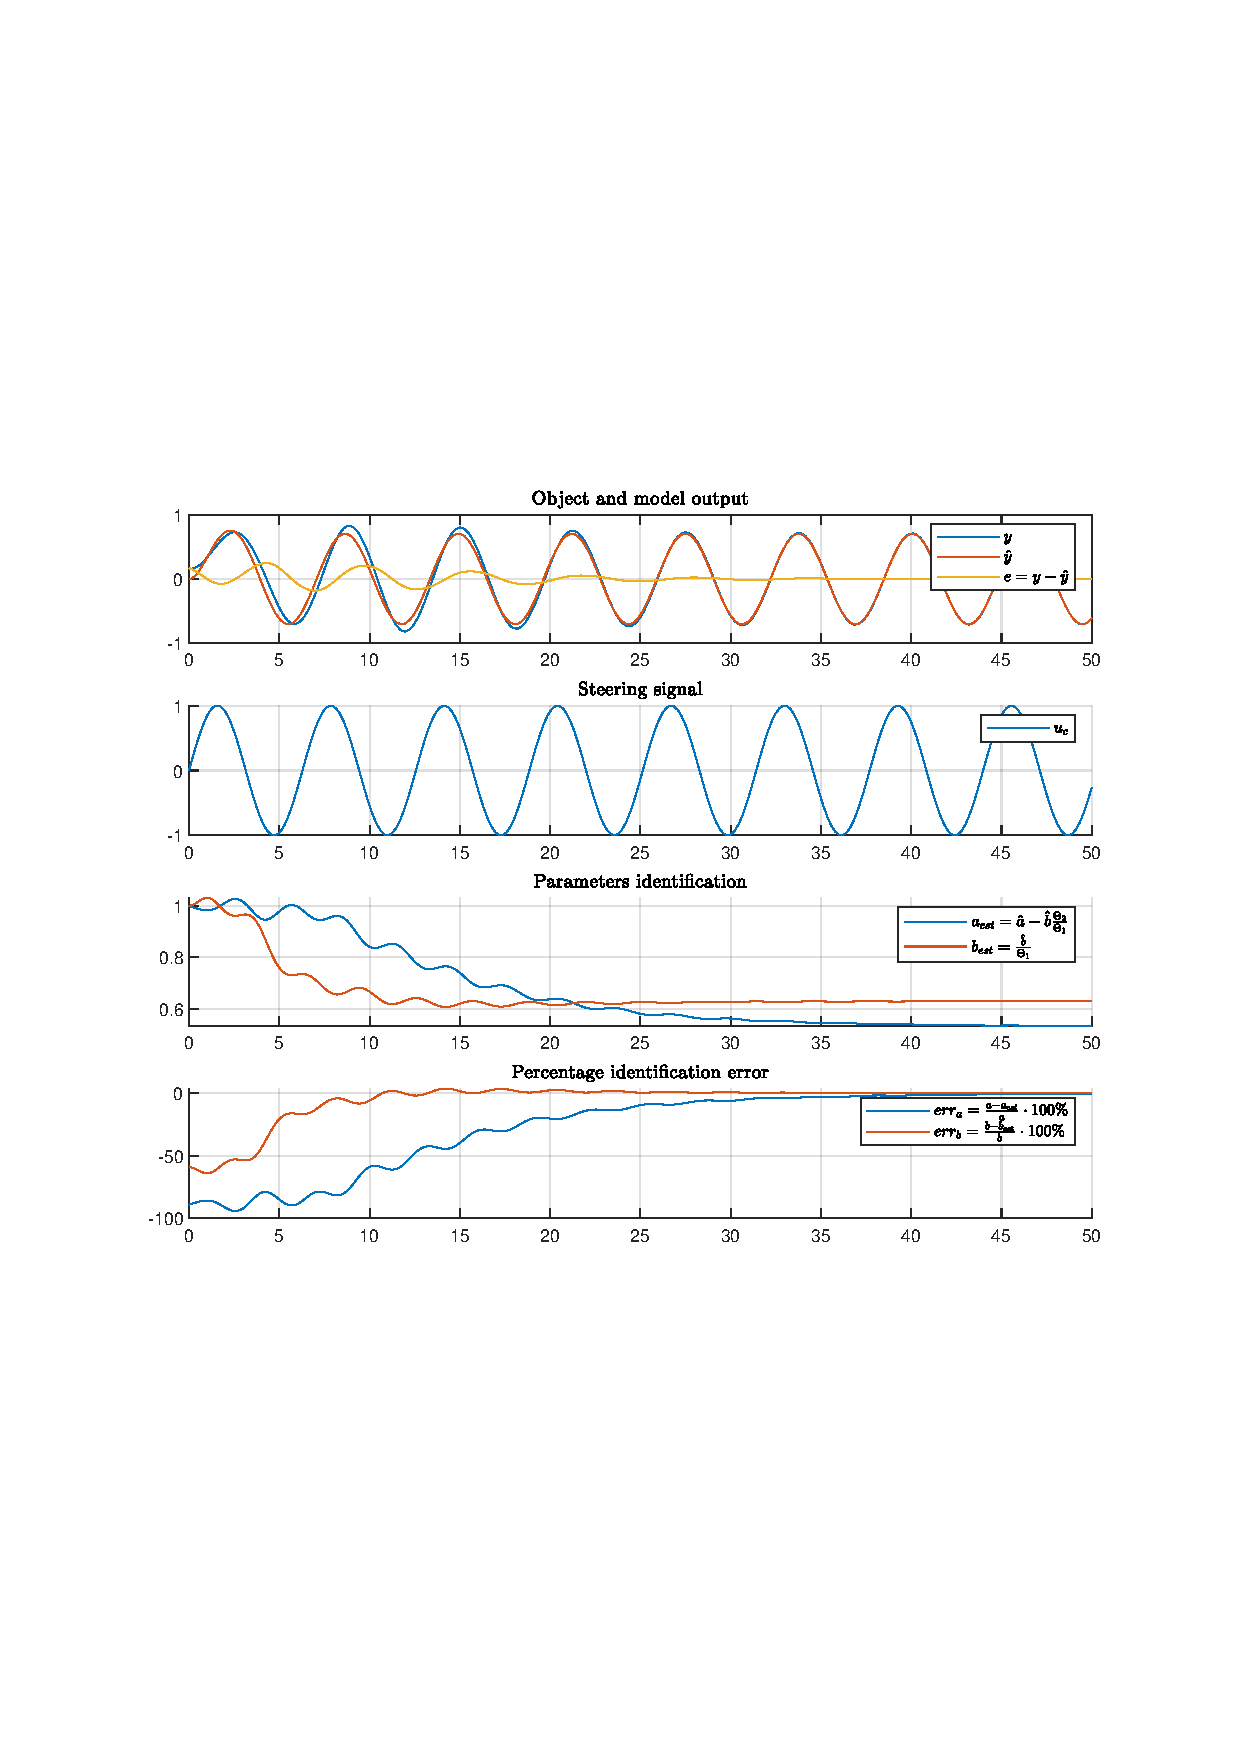
\includegraphics[width = 1.0\textwidth, trim = {0 8cm 0 8cm}]{sim.pdf}
\caption{Przebiegi sygna��w symulacji algorytmu identyfikacyjnego.}
\label{fig:sim}
\end{center}
\end{figure}







\end{document}